\subsection{The Haynes \& Shockley experiment}

Taking the measurements, we had to cope with various difficulties. 
Most notably, the observability of even the signal 
of the laser itself ceased at one point, probably due to the needle 
loosing contact or other technical issues. 
After trying to readjust the setup, we did observe a signal 
again. 
Only doing the evaluation did we notice that this also resulted in 
a large offset in time for all following measurements. 
Thus, the first four measurements have to be ignored. The offset 
remained stable for all but one ('File 7') of the further measurements. 
Furthermore, another set was so badly influenced by noise that 
a gaussian fit has no chance to converge. 
For the remaining data, we apply the following scheme: 
In order to facilitate the convergence of the fitting algorithm, 
we took the according set of smooth data, which is simply the 
average of 128 measurements done by the oscilloscope. 
The resulting parameters are then passed to the algorithm
as initial guesses for a fit on the original data. 
This is shown for an exemplary case in figure \ref{fig:h_s_raw_28}, 
where the measured distance between the point where the laser 
hits the material and the needle has been measured to 
$d = 3.7 \pm 0.5\,$mm. 
The parameters obtained by the fit with the original data 
are shown in a box within the plot as well. 
The fitted offset is omitted as it will not be used in any further 
calculation. The errors 
are obtained by the fitting algorithm as the square root of the 
diagonal entries. We did not further add an error on the 
$U$-value, as the scattering should be indication of 
uncertainty enough. For the oscilloscope, only 
a DC vertical accuracy is stated which would 
only apply for the offset. 
In the further calculations, we ignore the 
off-diagonal elements since the desired quantities each depend 
on only one parameter. 
Plots of all used data (original and smooth ones) with the 
fitted functions drawn are shown in the appendix, 
see~\ref{sec:appendix_h_s_plots}.
For all further calculations, the smoothed data is ignored 
and each calculation is done with the non-averaged ones. 
Errors will always be taken to be those of the fits.
An overview of the fitted parameters at corresponding 
distance $d$ is given in table~\ref{tab:h_s_fit_parameters}.

The obtained center of the gaussians $t_c$ are plotted over the 
according distances. With a linear fit, we calculate $\mu_c E$. 
The results are shown in figur~\ref{fig:h_s_fit_mu_e}. 



\renewcommand{\arraystretch}{1.5}
\begin{table}[htdp]
    \centering
    \caption{
        Results of fits with gaussians for all used data sets with distance 
        $d$ between laser and needle. The $\chi^2$-tests are quite high due to the 
        noise and tendencies to ascend on the scale of 10 sigma (compare figures, 
        e.~g.smooth data in figure~\ref{fig:h_s_raw_28}).
        }
    	\begin{tabular}{|p{2cm}|p{3cm}|p{3cm}|p{3cm}|p{2cm}|}
		\hline
		\rowcolor{tabcolor}
		$d \, / \, \mathrm{mm}$        & $A \, / \, \mathrm{\frac{mm}{\mu s}})$ & 
 			$t_c \, / \, \mathrm{\mu s}$    & $\sigma_t \, / \, \mathrm{\mu s}$ & 
 			$\chi^2 / n_d$ \\ \hline
		$7.5$ & $3.2 \pm 0.2$ & $377.54 \pm 0.13$ & $1.93 \pm 0.13$ & $10.2$\\ 
		$8.5$ & $3.3 \pm 0.3$ & $378.28 \pm 0.20$ & $1.98 \pm 0.20$ & $3.0$\\ 
		$8.0$ & $2.5 \pm 0.3$ & $377.58 \pm 0.20$ & $1.69 \pm 0.20$ & $2.8$\\ 
		$7.5$ & $2.7 \pm 0.2$ & $376.50 \pm 0.11$ & $1.23 \pm 0.11$ & $2.6$\\ 
		$5.9$ & $3.0 \pm 0.2$ & $372.45 \pm 0.09$ & $1.05 \pm 0.09$ & $3.4$\\ 
		$4.4$ & $4.0 \pm 0.2$ & $368.91 \pm 0.05$ & $1.14 \pm 0.05$ & $9.9$\\ 
		$3.9$ & $3.8 \pm 0.2$ & $367.71 \pm 0.05$ & $1.12 \pm 0.05$ & $12.3$\\ 
		$3.7$ & $6.3 \pm 0.2$ & $367.09 \pm 0.04$ & $1.37 \pm 0.04$ & $12.3$\\ 
		$1.1$ & $12.2 \pm 0.2$ & $362.66 \pm 0.01$ & $0.95 \pm 0.01$ & $12.3$\\ 
		\hline
	\end{tabular}

    \label{tab:h_s_fit_parameter}
\end{table}

\begin{figure}
    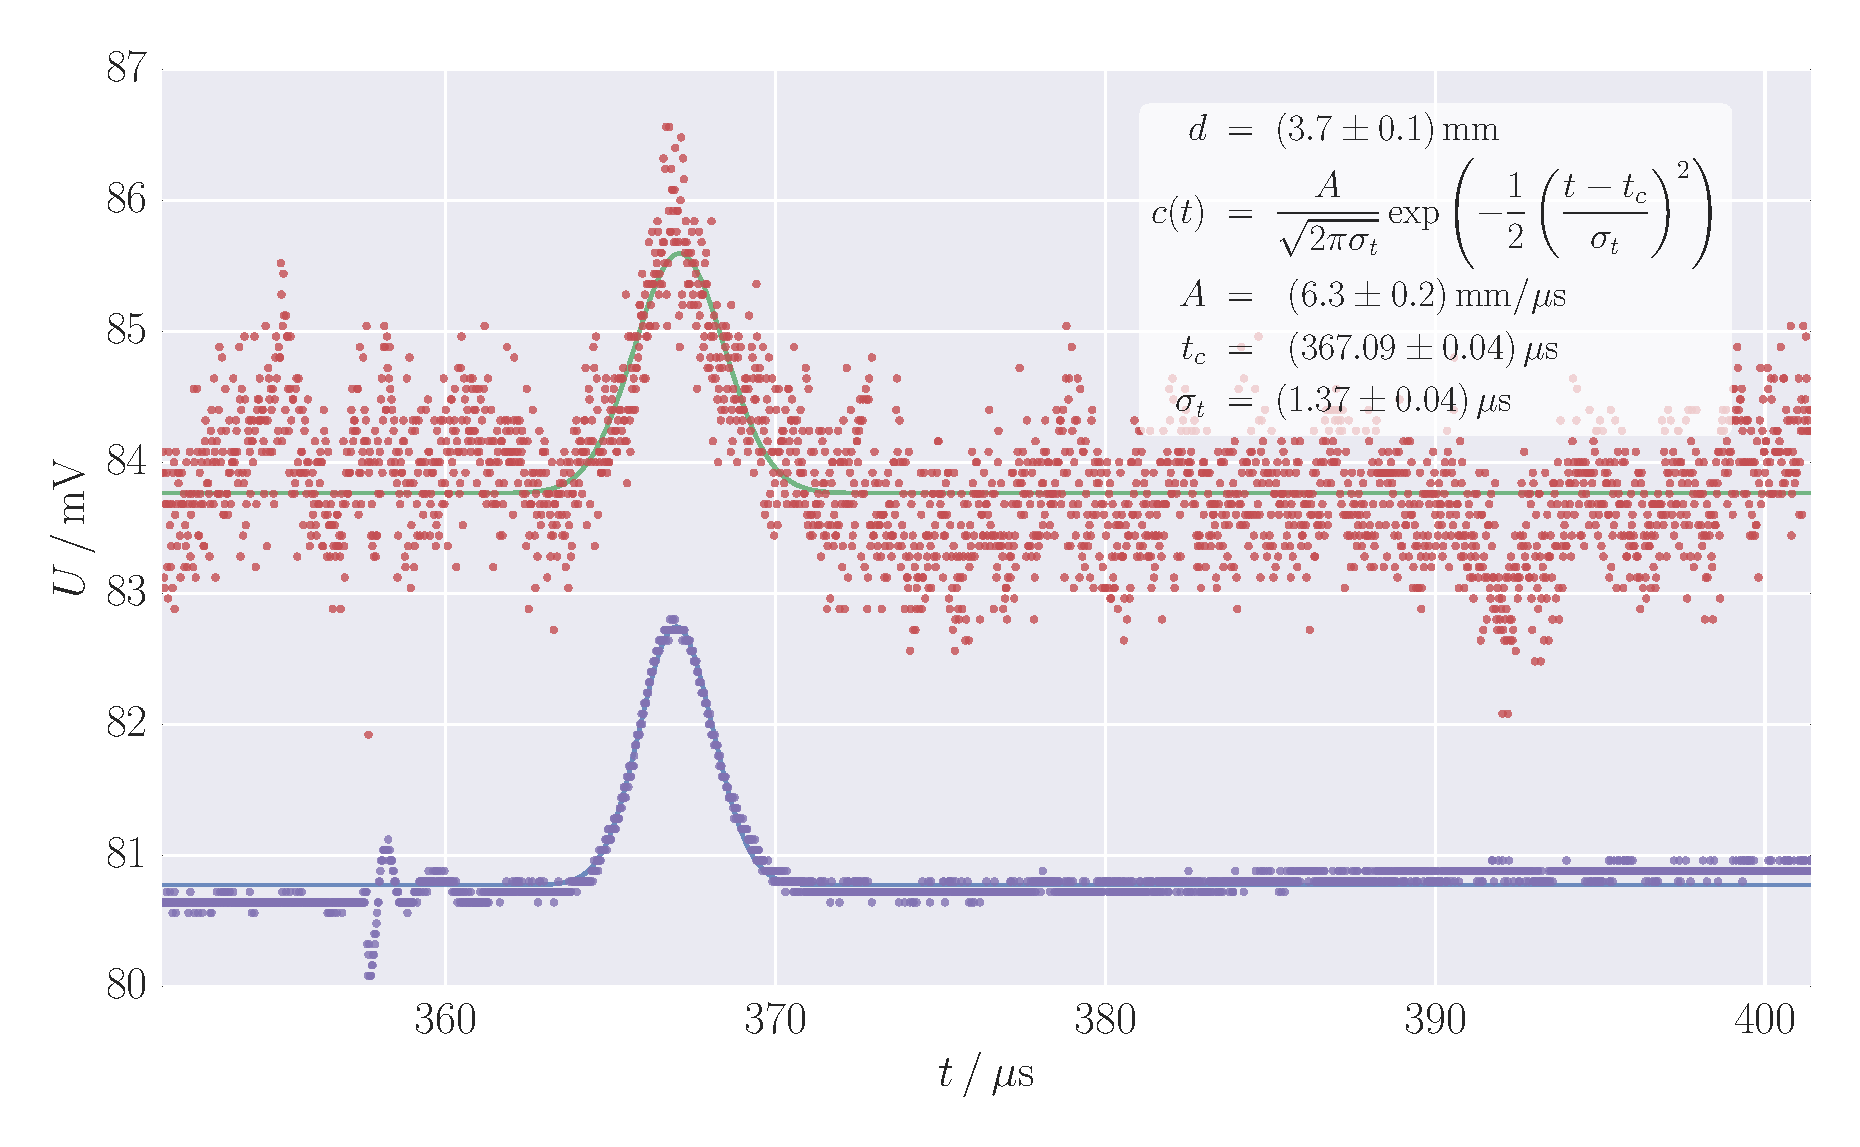
\includegraphics[width=1.0\textwidth]{figures/haynes_shockley_raw_28}
    \caption{
        Raw data and fitted gaussians for $d = 3.7 \pm 0.5\,$cm. 
        The lower, much more scattered data is taken without averaging 
        while the upper corresponds to the average of 128 measurements, where the 
        running average is done by the oscilloscope directly. This smoother data is 
        used to obtain the guesses for the fit on the noisy data, 
        while all further calculations are done with the original, 
        non-averaged data. 
        One can observe the large offset which is of unknown origin appearing 
        after a temporary loss of signal and small adjustments on the setup.
        }
    \label{fig:h_s_raw_28}
\end{figure}

\begin{figure}
    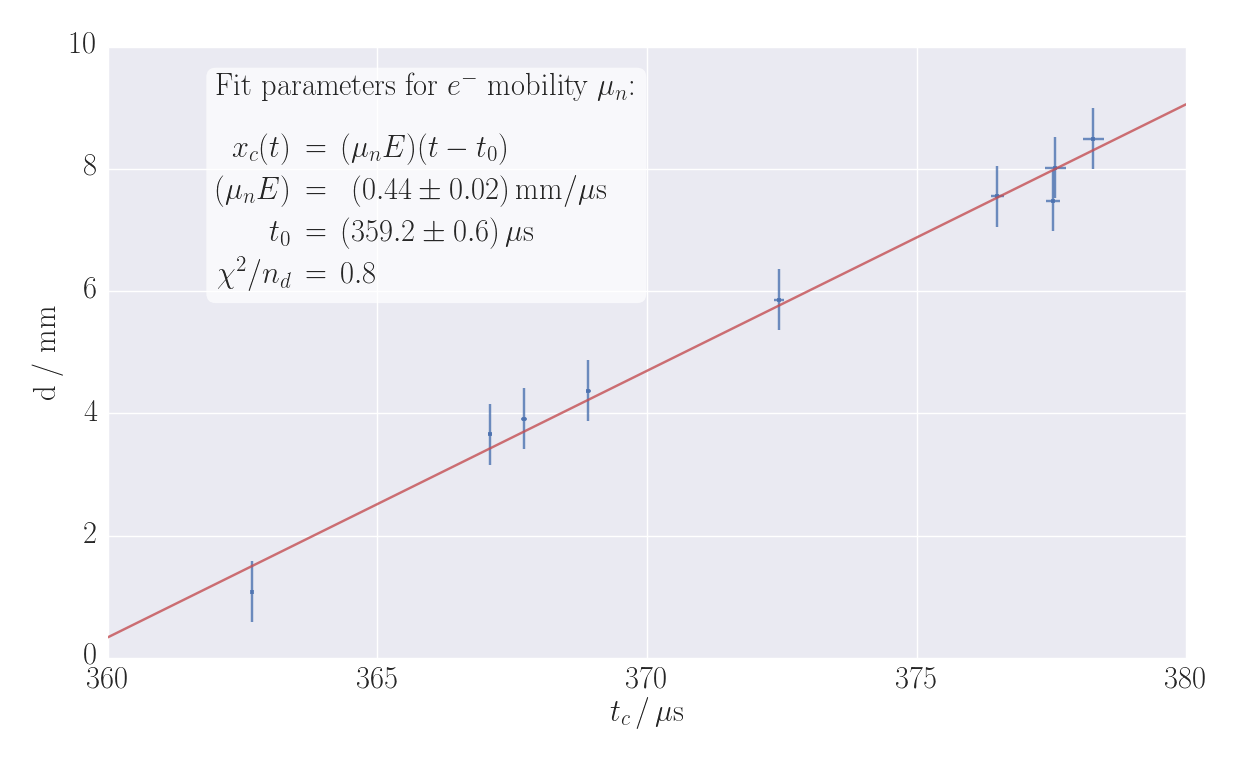
\includegraphics[width=1.0\textwidth]{figures/haynes_shockley_mu_e}
    \caption{
        Fitted straight line on centers of gaussians as calculated before. 
        The linear behavior is see quite well, as indicated also by the 
        $\chi^2$-test.
        }
    \label{fig:h_s_mu_e}
\end{figure}

